% uWaterloo Thesis Template for LaTeX 
% Last Updated May 24, 2011 by Stephen Carr, IST Client Services
% FOR ASSISTANCE, please send mail to rt-IST-CSmathsci@ist.uwaterloo.ca

% Effective October 2006, the University of Waterloo 
% requires electronic thesis submission. See the uWaterloo thesis regulations at
% http://www.grad.uwaterloo.ca/Thesis_Regs/thesistofc.asp.

% DON'T FORGET TO ADD YOUR OWN NAME AND TITLE in the "hyperref" package
% configuration below. THIS INFORMATION GETS EMBEDDED IN THE PDF FINAL PDF DOCUMENT.
% You can view the information if you view Properties of the PDF document.

% Many faculties/departments also require one or more printed
% copies. This template attempts to satisfy both types of output. 
% It is based on the standard "book" document class which provides all necessary 
% sectioning structures and allows multi-part theses.

% DISCLAIMER
% To the best of our knowledge, this template satisfies the current uWaterloo requirements.
% However, it is your responsibility to assure that you have met all 
% requirements of the University and your particular department.
% Many thanks to the feedback from many graduates that assisted the development of this template.

% -----------------------------------------------------------------------

% By default, output is produced that is geared toward generating a PDF 
% version optimized for viewing on an electronic display, including 
% hyperlinks within the PDF.
 
% E.g. to process a thesis called "mythesis.tex" based on this template, run:

% pdflatex mythesis	-- first pass of the pdflatex processor
% bibtex mythesis	-- generates bibliography from .bib data file(s) 
% pdflatex mythesis	-- fixes cross-references, bibliographic references, etc
% pdflatex mythesis	-- fixes cross-references, bibliographic references, etc

% If you use the recommended LaTeX editor, Texmaker, you would open the mythesis.tex
% file, then click the pdflatex button. Then run BibTeX (under the Tools menu).
% Then click the pdflatex button two more times. If you have an index as well,
% you'll need to run MakeIndex from the Tools menu as well, before running pdflatex
% the last two times.

% N.B. The "pdftex" program allows graphics in the following formats to be
% included with the "\includegraphics" command: PNG, PDF, JPEG, TIFF
% Tip 1: Generate your figures and photos in the size you want them to appear
% in your thesis, rather than scaling them with \includegraphics options.
% Tip 2: Any drawings you do should be in scalable vector graphic formats:
% SVG, PNG, WMF, EPS and then converted to PNG or PDF, so they are scalable in
% the final PDF as well.
% Tip 3: Photographs should be cropped and compressed so as not to be too large.

% To create a PDF output that is optimized for double-sided printing: 
%
% 1) comment-out the \documentclass statement in the preamble below, and
% un-comment the second \documentclass line.
%
% 2) change the value assigned below to the boolean variable
% "PrintVersion" from "false" to "true".

% --------------------- Start of Document Preamble -----------------------

% Specify the document class, default style attributes, and page dimensions
% For hyperlinked PDF, suitable for viewing on a computer, use this:
\documentclass[letterpaper,12pt,titlepage,oneside,final]{book}
 
% For PDF, suitable for double-sided printing, change the PrintVersion variable below
% to "true" and use this \documentclass line instead of the one above:
%\documentclass[letterpaper,12pt,titlepage,openright,twoside,final]{book}

% Some LaTeX commands I define for my own nomenclature.
% If you have to, it's better to change nomenclature once here than in a 
% million places throughout your thesis!
\newcommand{\package}[1]{\textbf{#1}} % package names in bold text
\newcommand{\cmmd}[1]{\textbackslash\texttt{#1}} % command name in tt font 
\newcommand{\href}[1]{#1} % does nothing, but defines the command so the
    % print-optimized version will ignore \href tags (redefined by hyperref pkg).
%\newcommand{\texorpdfstring}[2]{#1} % does nothing, but defines the command
% Anything defined here may be redefined by packages added below...

% This package allows if-then-else control structures.
\usepackage{ifthen}
\newboolean{PrintVersion}
\setboolean{PrintVersion}{false} 
% CHANGE THIS VALUE TO "true" as necessary, to improve printed results for hard copies
% by overriding some options of the hyperref package below.

%\usepackage{nomencl} % For a nomenclature (optional; available from ctan.org)
\usepackage{amsmath,amssymb,amstext} % Lots of math symbols and environments
\usepackage[pdftex]{graphicx} % For including graphics N.B. pdftex graphics driver 

\usepackage[chapter]{algorithm}
\usepackage{algorithmic}
% Hyperlinks make it very easy to navigate an electronic document.
% In addition, this is where you should specify the thesis title
% and author as they appear in the properties of the PDF document.
% Use the "hyperref" package 
% N.B. HYPERREF MUST BE THE LAST PACKAGE LOADED; ADD ADDITIONAL PKGS ABOVE
\usepackage[pdftex,letterpaper=true,pagebackref=false]{hyperref} % with basic options
		% N.B. pagebackref=true provides links back from the References to the body text. This can cause trouble for printing.
\hypersetup{
    plainpages=false,       % needed if Roman numbers in frontpages
    pdfpagelabels=true,     % adds page number as label in Acrobat's page count
    bookmarks=true,         % show bookmarks bar?
    unicode=false,          % non-Latin characters in Acrobat’s bookmarks
    pdftoolbar=true,        % show Acrobat’s toolbar?
    pdfmenubar=true,        % show Acrobat’s menu?
    pdffitwindow=false,     % window fit to page when opened
    pdfstartview={FitH},    % fits the width of the page to the window
    pdftitle={uWaterloo\ LaTeX\ Thesis\ Template},    % title: CHANGE THIS TEXT!
%    pdfauthor={Author},    % author: CHANGE THIS TEXT! and uncomment this line
%    pdfsubject={Subject},  % subject: CHANGE THIS TEXT! and uncomment this line
%    pdfkeywords={keyword1} {key2} {key3}, % list of keywords, and uncomment this line if desired
    pdfnewwindow=true,      % links in new window
    colorlinks=true,        % false: boxed links; true: colored links
    linkcolor=blue,         % color of internal links
    citecolor=green,        % color of links to bibliography
    filecolor=magenta,      % color of file links
    urlcolor=cyan           % color of external links
}
\ifthenelse{\boolean{PrintVersion}}{   % for improved print quality, change some hyperref options
\hypersetup{	% override some previously defined hyperref options
%    colorlinks,%
    citecolor=black,%
    filecolor=black,%
    linkcolor=black,%
    urlcolor=black}
}{} % end of ifthenelse (no else)

% Setting up the page margins...
% uWaterloo thesis requirements specify a minimum of 1 inch (72pt) margin at the
% top, bottom, and outside page edges and a 1.125 in. (81pt) gutter
% margin (on binding side). While this is not an issue for electronic
% viewing, a PDF may be printed, and so we have the same page layout for
% both printed and electronic versions, we leave the gutter margin in.
% Set margins to minimum permitted by uWaterloo thesis regulations:
\setlength{\marginparwidth}{0pt} % width of margin notes
% N.B. If margin notes are used, you must adjust \textwidth, \marginparwidth
% and \marginparsep so that the space left between the margin notes and page
% edge is less than 15 mm (0.6 in.)
\setlength{\marginparsep}{0pt} % width of space between body text and margin notes
\setlength{\evensidemargin}{0.125in} % Adds 1/8 in. to binding side of all 
% even-numbered pages when the "twoside" printing option is selected
\setlength{\oddsidemargin}{0.125in} % Adds 1/8 in. to the left of all pages
% when "oneside" printing is selected, and to the left of all odd-numbered
% pages when "twoside" printing is selected
\setlength{\textwidth}{6.375in} % assuming US letter paper (8.5 in. x 11 in.) and 
% side margins as above
\raggedbottom

% The following statement specifies the amount of space between
% paragraphs. Other reasonable specifications are \bigskipamount and \smallskipamount.
\setlength{\parskip}{\medskipamount}

% The following statement controls the line spacing.  The default
% spacing corresponds to good typographic conventions and only slight
% changes (e.g., perhaps "1.2"), if any, should be made.
\renewcommand{\baselinestretch}{1} % this is the default line space setting

% By default, each chapter will start on a recto (right-hand side)
% page.  We also force each section of the front pages to start on 
% a recto page by inserting \cleardoublepage commands.
% In many cases, this will require that the verso page be
% blank and, while it should be counted, a page number should not be
% printed.  The following statements ensure a page number is not
% printed on an otherwise blank verso page.
\let\origdoublepage\cleardoublepage
\newcommand{\clearemptydoublepage}{%
  \clearpage{\pagestyle{empty}\origdoublepage}}
\let\cleardoublepage\clearemptydoublepage

%======================================================================
%   L O G I C A L    D O C U M E N T -- the content of your thesis
%======================================================================
\begin{document}

% For a large document, it is a good idea to divide your thesis
% into several files, each one containing one chapter.
% To illustrate this idea, the "front pages" (i.e., title page,
% declaration, borrowers' page, abstract, acknowledgements,
% dedication, table of contents, list of tables, list of figures,
% nomenclature) are contained within the file "uw-ethesis-frontpgs.tex" which is
% included into the document by the following statement.
%----------------------------------------------------------------------
% FRONT MATERIAL
%----------------------------------------------------------------------
% T I T L E   P A G E
% -------------------
% Last updated May 24, 2011, by Stephen Carr, IST-Client Services
% The title page is counted as page `i' but we need to suppress the
% page number.  We also don't want any headers or footers.
\pagestyle{empty}
\pagenumbering{roman}

% The contents of the title page are specified in the "titlepage"
% environment.
\begin{titlepage}
        \begin{center}
        \vspace*{1.0cm}

        \Huge
        {\bf Visual Object Tracking with Deep Q Networks }

        \vspace*{1.0cm}

        \normalsize
        by \\

        \vspace*{1.0cm}

        \Large
        Michael Noukhovitch \\

        \vspace*{3.0cm}

        \normalsize
        A report \\
        presented to the University of Waterloo \\ 
        in fulfillment of the \\
        report requirement for SE 499 \\

        \vspace*{2.0cm}

        Waterloo, Ontario, Canada, 2016 \\

        \vspace*{1.0cm}

        \copyright\ Michael Noukhovitch 2016 \\
        \end{center}
\end{titlepage}

% The rest of the front pages should contain no headers and be numbered using Roman numerals starting with `ii'
\pagestyle{plain}
\setcounter{page}{2}

\cleardoublepage % Ends the current page and causes all figures and tables that have so far appeared in the input to be printed.
% In a two-sided printing style, it also makes the next page a right-hand (odd-numbered) page, producing a blank page if necessary.
 


% D E C L A R A T I O N   P A G E
% -------------------------------
  % The following is the sample Delaration Page as provided by the GSO
  % December 13th, 2006.  It is designed for an electronic thesis.
  \noindent
I hereby declare that I am the sole author of this report. This is a true copy of the report, including any required final revisions, as accepted by my examiners.

  \bigskip
  
  \noindent
I understand that my report may be made electronically available to the public.

\cleardoublepage
%\newpage

% A B S T R A C T
% ---------------

\begin{center}\textbf{Abstract}\end{center}

This is the abstract.

ABSTRACT
ABSTRACT
ABSTRACT
ABSTRACT
ABSTRACT


\cleardoublepage
%\newpage

% A C K N O W L E D G E M E N T S
% -------------------------------

\begin{center}\textbf{Acknowledgements}\end{center}

I would like to thank Pascal Poupart, my advisor, as well as Daniel Que, a student I worked alongside during SE 499. As well, I'd like to thank the Waterloo AI lab (MATLAB) for being nice and welcoming.
\cleardoublepage
%\newpage


% T A B L E   O F   C O N T E N T S
% ---------------------------------
\renewcommand\contentsname{Table of Contents}
\tableofcontents
\cleardoublepage
\phantomsection
%\newpage

% L I S T   O F   T A B L E S
% ---------------------------
%\addcontentsline{toc}{chapter}{List of Tables}
%\listoftables
%\cleardoublepage
%\phantomsection		% allows hyperref to link to the correct page
% -- %\newpage

% L I S T   O F   F I G U R E S
% -----------------------------
\addcontentsline{toc}{chapter}{List of Figures}
\listoffigures
\cleardoublepage
\phantomsection		% allows hyperref to link to the correct page
%\newpage

% L I S T   O F   A L G O R I T H M S
% -----------------------------
\addcontentsline{toc}{chapter}{List of Algorithms}
\listofalgorithms
\cleardoublepage
\phantomsection		% allows hyperref to link to the correct page
%\newpage

% L I S T   O F   S Y M B O L S
% -----------------------------
% To include a Nomenclature section
% \addcontentsline{toc}{chapter}{\textbf{Nomenclature}}
% \renewcommand{\nomname}{Nomenclature}
% \printglossary
% \cleardoublepage
% \phantomsection % allows hyperref to link to the correct page
% \newpage

% Change page numbering back to Arabic numerals
\pagenumbering{arabic}

 

%----------------------------------------------------------------------
% MAIN BODY
%----------------------------------------------------------------------
% Because this is a short document, and to reduce the number of files
% needed for this template, the chapters are not separate
% documents as suggested above, but you get the idea. If they were
% separate documents, they would each start with the \chapter command, i.e, 
% do not contain \documentclass or \begin{document} and \end{document} commands.
%======================================================================
\chapter{Introduction}
Artificial intelligence (or machine learning as it can be called) is a thriving field that applies intelligent algorithms to difficult problems and automate tasks. Early on, these problems were those that were difficult for humans but easy for machines. Now there has been a trend of having computers automate very human tasks that were previously deemed impossible for computers \cite{deep-learning-book}. Computer vision is in line with this train of thought and deals with teaching computers to recognize and understand visuals. Visual object tracking, the question put forth here, is a computer vision task that aims to track a visual object over time (e.g. in a video). This difficult task has had great breakthroughs recently, due to the effectiveness of deep neural networks. This report explores using deep neural networks in intelligent ways to solve the task.

\chapter{Background Information}
\section{Deep Neural Networks}
The basis of deep learning, the technology used, is neural networks. These are architectures that ``learn to map a fixed-size input (for example, an image) to a fixed-size output (for example, a probability for each of several categories)'' \cite{deep-learning-article}. They do so by having ``layers'' of neurons where each neuron is a function on its input (usually the output of the previous layer). By feeding forward the inputs through many layers, complex features can be extracted by the network using interesting combinations of neurons. 

\begin{figure}
	\centering
	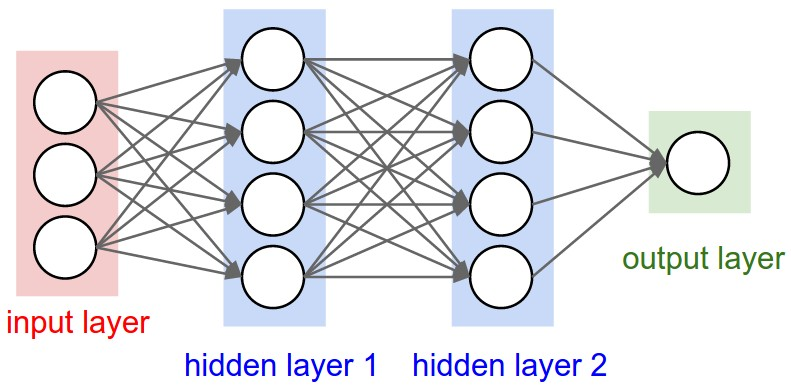
\includegraphics[scale=0.3]{neural_net}
	\caption{basic example of a neural network \cite{cs231n}}
\end{figure}

By using the property that complex features tend to be built on top of simple features (e.g. using lines to form shapes), we find that having many layers of neurons allow us to learn to disinguish more and more complex features at the deeper layers \cite{deep-learning-article}. This idea, that complex features learned as a deeper layer of simple features, forms the basis for our approach to visual classification. 

\section{Convolutional Neural Networks}
Just using normal neurons in combination is an effective but expensive strategy for images. If each neuron has a function that uses one weight variable per input (e.g. output is some weighted sum of inputs) then we can quickly get overwhelmed. For example, if we have a \textit{fully connected} layer where each neuron is connected to each input, then for an image of a measly size of 32 pixels wide x 32 pixels tall x 3 colour channels (RGB), we already have 3072 weights in every input neuron! This is a very small image and more weights means more difficulty to train as well as overfitting. To this end, we use \textit{convolutional} layers to decrease the number of parameters (weights) while still processing the input. 


Based on the concept of a ``sliding window'' that slides over a whole image, we create a \textit{filter} that will be our sliding window and assign it only as many weights as it needs (5x5 filter $\rightarrow$ 5x5x3 (RGB) = 75 weights). We then use this filter over the whole image and thus save on parameters \cite{cs231n}. We also get the benefit of locality since our window looks at groups of pixels at a time. This means that it doesn't matter where in the image our pixels are, as long as our sliding window passes over them it acts as the same input, meaning we have translational invariance.

\begin{figure}[b]
	\centering
	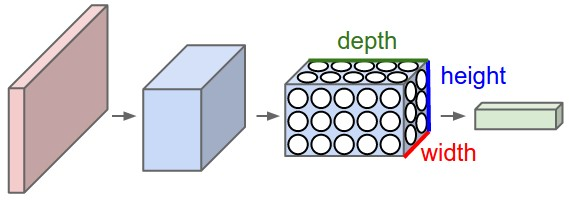
\includegraphics[scale=0.3]{conv}
	\caption{basic example of a convolutional network \cite{cs231n}}
\end{figure}

These benefits, among others, mean that convolutional neural networks are excellent for processing images and indeed are the basis of the state of the art image object classification, video object classification, scene classification, and more \cite{ILSVRC15} \cite{resnet}.


\section{Reinforcement Learning}
This research also makes use of another large field in machine learning, reinforcement learning. ``Reinforcement learning is learning what to do--how to map situations to actions--so as to maximize a numerical reward signal.'' \cite{sutton-barto} We start by modelling situations as Markov decision processes, where we specify each component of a task by modelling everything including uncertainty. We can say that a task is at a current state $s$ that is one of the possible states in the state space $S$. As well, we can take an action $a$ from this state (part of action space $A$) and recieve a reward for this action $r$ \cite{pascal-mdp}.


\begin{figure}[h]
	\centering
	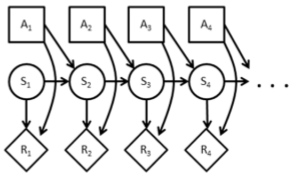
\includegraphics[scale=1.0]{mdp}
	\caption{graphical model representation of an mdp\cite{pascal-mdp}}
\end{figure}

We can also add the horizon $h$ which specifies how far into the future out agent should plan, and the discount factor $\gamma$ which determines how to weigh rewards at different steps in time, specifically, how the rewards decrease at later time steps.


Reinforcement learning deals with finding a policy $\pi$ that will maximize our reward by choosing an action at every time step, which ends up being maximizing the ``expected sum of discounted rewards earned while executing the policy'' \cite{pascal-mdp}, for a value function $V^\pi(s)$

\begin{equation}
	V^\pi(s) = \sum_{t=0}^{\infty} \gamma^{t}E_{\pi}[R(s_t, \pi(s_t))] \forall s
\end{equation}

rewriting the value function to be recursive as the sum of the current reward and discounted future rewards

\begin{equation}
	V^\pi(s) = R(s, \pi(s)) + \gamma \sum_{s'} Pr(s'|s, \pi(s)) V^\pi(s') \forall s
\end{equation}

an optimal policy is one that maximizes $V^\pi (s)$, so one where $V^{\pi *}(s) \ge V^{\pi}(s) \ \forall s, \pi$ \cite{pascal-mdp}, which means it will satisfy Bellaman's equation

\begin{equation}
	V^{\pi *}(s) = \max_{a} R(s, a) + \gamma \sum_{s'} Pr(s'|s, \pi(s)) V^{\pi *}(s') \forall s
\end{equation}


The question then becomes how do we find this policy $\pi$, especially if the probabilities or rewards are known only for some states? There are many approaches, but a simple one is value iteration. Value iteration which uses dynamic programming to optimize the values from the last time step and works backwards. Eventually, you arrive at the maximal value at each time step $t$ and can find the optimal policy $\pi$. Another approach involves using monte-carlo methods instead of dynamic programming and yet other approach use temporal-difference learning. These learning methods learn from raw experience without a model (much like Monte Carlo methods) but also update their estimates of the solution as they go, bootstrapping in a sense \cite{sutton-barto}.

One temporal learning algorithm that we will use is called ``Q-learning''. This algorithm seeks to find an approximator to the optimal quality function $Q*$ which maps between state, action pairs and their value \cite{sutton-barto}. Using our approximation $Q$, we can then select the action which will lead to the highest value for this state and our policy is done! Formally, Q-learning can be written as 

\begin{equation}
	Q(s_t, a_t) \leftarrow Q(s_t, a_t) + \alpha [r_{t+1} + \gamma \max_{a} Q(s_{t+1}, a) - Q(s_t, a_t)] \cite{sutton-barto}
\end{equation}

Where $\alpha$ is the learning rate, used to stochastically update $Q$. This equation just means that $Q$ is stochastically updated as it goes, with the improved policy at each state-action pair. The policy doesn't affect how the updates are made, $Q$ is updated independent of the policy, but it does determine the order in which state-action pairs are visited and updated \cite{sutton-barto}.

\section{Deep Reinforcement Learning}
The fields of deep learning and reinforcement learning were somewhat distinct and separate until certain breakthroughs showed that combining them can lead to powerful algorithms. Deep reinforcement learning as done in \cite{atari-dqn} combines deep convolutional neural networks and q-learning to create a system that learns actions from raw image/video input. By saving the experiences of the agent in a dataset, called \textit{replay memory}, we can train the neural network on batches of inputs and values to allow for learning both the Q-function and weights of the neural network at the same time. Formally the algorithm is called \textit{deep Q-learning} and since using histories of different lengths can be difficult, we looks at fixed length representations of histories produced by a function $\phi$ \cite{atari-dqn}. 


\begin{algorithm}
\caption{Deep Q-Learning with Experience Replay \cite{atari-dqn}}
\label{dqn-algorithm}
\begin{algorithmic}
\STATE Initialize replay memory $D$ to capacity $N$
\STATE Initialize action-value function $Q$ with random weights
\FOR{episode=1 \TO M} 
\STATE Initialize sequence $s_1 = {x_1}$ and preprocessed $\phi_1 = \phi(s_1)$
\FOR{t=1 \TO $T$}
\STATE With probability $\eta$ select a random action $a_t$
\STATE otherwise select $a_t = \max_{a} Q^*(\phi(s_t), a; \Theta)$
\STATE Execute action $a_t$ in emulator and observe reward $r_t$ and image $x_{t+1}$ 
\STATE Set $s_{t+1} = s_t, a_t, x_{t+1}$ and preprocess $\phi_{t+1} = \phi(s_{t+1})$
\STATE Store transition $(\phi_t, a_t, r_t, \phi_{t+1})$ in $D$
\STATE Sample random minibatch of transitions $(\phi_j, a_j, r_j, \phi_{j+1})$ from $D$
\STATE Set $ y_j =
	\begin{cases} 
		r_j & \text{ for terminal } \phi_{j+1} \\
		r_j + \gamma \max_{a'} Q(\phi_{j+1}, a'; \Theta) & \text{ for non-terminal } \phi_{j+1}
	\end{cases}
		$
\STATE Perform a gradient descent step on $(y_j - Q(\phi_j, a_j; \Theta))^2$ according the Q-learning algorithm
\ENDFOR
\ENDFOR
\end{algorithmic}
\end{algorithm}

This algorithm was used for playing Atari video game based on the last four frames of a current state, but we will be applying it to visual object tracking in a similar manner.


\chapter{The Problem}
\section{Visual Object Tracking}
The challenge set forth is \textit{visual object tracking}, which is a research area pursued in many different ways. The core of this task is to keep track of an object in a video over the length of the video. Many different datasets and approaches exist but a popular one that has emerged is the Visual Object Tracking challenge, most recently done in coordination with International Conference on Computer Vision (ICCV2015). This challenge standardizes the visual tracking task as one that ``considers single-camera, single-target, model-free, causal trackers, applied to short-term tracking'' \cite{vot2015}. Breaking that down, single camera implies that the input is a continuous video taken from a single camera (though the camera can move). Single target means that there is only one object to be tracked in the video. Model-free means that ``the only supervised training example is provided by the bounding box in the first frame'' \cite{vot2015}, so the object can be anything and the input given is just a visual cue of where in the first frame the object is. Causal tracking means that the tracker can't use future frames or frames prior to re-initialization to detect the object. Finally, short-term implies that the tracker does not re-detect the object if the target is lost; drifting off of the target is considered failure.


With all these restrictions put into place, we end up with a fairly narrow and precise goal. Also useful, is that the VOT challenge provides labelled training data and this work will be using the most recent VOT 2016 training data which consists of 60 videos each containing somewhere between 50 and 1000 frames with the average being somewhere in the 300s. Each video is labelled at every frame with a rectangular bounding box known as the \textit{ground truth}. Extra labels on the video are also provided as booleans for every frame: camera motion, illumination change, motion change, object size change. 

\section{Related Work}

Since the VOT challenge has been running for three years now, there have already been many approaches to this problem from combined approaches that used traditional statistical machine learning such as kernelized correlation features (KCF) \cite{kcf} to more recent approaches using neural networks \cite{mdnet}. VOT2015 saw many different approaches ultimately having neural networks be a part of many of the more successful entries \cite{vot2015}.

One particularly interesting entry was the eventual contest-winner MDNet, which used a fairly standard convolutional network that reserved a final fully-connected layer for tracking specific to that video (referred to as the \textit{domain} as MDNet stands for``Multi-Domain Network'') \cite{mdnet}. The simple but effective convolutional layers already produced excellent results and combined with domain-specific final layers, made for a robust and accurate network. Since VOT2015 measured the networks by finding the expected average overlap between the ground truth bounding boxes and the output of the network, this robustness as well as accuracy managed to make up for he lack of speed in the network, crowning MDNet the winner \cite{vot2015}. These results are encouraging to our use of convolutional neural networks.


\chapter{The Approach}
\section{DQN for Visual Object Tracking}
The novel approach suggested here is to use the same type of network as in \cite{atari-dqn} for the purposes of visual object tracking on the VOT2016 dataset. The setup will be similar to the DQN proposed only we don't have any need for experience replay as our dataset is not a game that must be played through online but a set of videos from which we can sample. 

We will model the bounding box as our state and actions will be modifications to the bounding box. Possible actions are then, translation in x, translation in y, changing the size of the bounding box in x, changing the size of the bounding box in y (we will not count rotations as our bounding boxes should always we upright). In this way there are 8 possible actions (left, right, up, down, and shrink/grow for each direction).

Modelling the reward is tricky but we will use a common bounding box measure over intersect over union (IoU) to find the reward. This is the measure of how close our estimated bounding box is to the ground truth. We measure the area in the intersection of the two bounding boxes and divide it by the area of the union of the two bounding boxes. In the ideal case, where our box matches perfectly with the ground truth, we find that IoU = 1. In the case that we lose complete track of our ground truth, we have IoU = 0. In this way, we make the reward function equal to the IoU, hoping that our estimate bounding box will cover as much as possible of the ground truth and as little else as possible.

This situation is a little bit interesting in that we really don't need a $\gamma$ because the ground truth labels are available at every time step and every time step is just as important for the task of tracking. We can still experiment, though, with using a different horizon and different sampling techniques (e.g. taking a 10 frame clip regardless of which video). The input though, is similar to the DQN in \cite{atari-dqn} as it uses a concatenation of four frames (to get a sense of motion) instead of just using a single frame.

Intuitively, it can be thought of as moving the bounding box at each time step (frame) to be in line with the ground truth bounding box. Theoretically, this approach should win over other approaches that seek to redraw the bounding box from scratch at every frame, since we would require much fewer bits of information per each new frame and would literally be ``tracking'' the visual cues over time.

\section{Implementation}
The implementation is done in Tensorflow for scalability and future-proofing reasons. Input videos (series of frames) are converted into tfrecords files and fed into the network using parallelized input queues. Batches can be shuffled and split among many different devices, and GPU support is available for the network. Tensorflow can also be a bit verbose, so a high-level library, Tensorflow-Slim, is used to make networks as well as other code more readable. This has the added benefit of automatically integrating into Tensorflow's visualization library Tensorboard, which allows for real-time visualization of various metrics and variables during training and testing. As well, due to the parallizable nature of Tensorflow-Slim, both training and evaluation can happen simulataneously allowing for faster training and a better understanding of overfitting in the network (also possible to view output activations to check for overfitting).

Sadly, there are no good deep Q-learning implementation available online. All implementations tend to be very application specific (e.g. DQN for Atari in lua for \cite{atari-dqn}) but nothing that can interface well and in a modular fashion. The main issue is that the algorithm itself is very new and most professional implementations that would be tied to Tensorflow are most likely exclusively available within private companies (Google, Deepmind\dots). This means that I have had to put together my own implementation of a deep Q network from various sources online.

\section{Possible Drawbacks}
One major criticism that can be used is that reinforcement learning is overkill for this exact problem. Reinforcement learning excels at learning from rewards that are not directly related to each individual action (e.g. in pong, the paddle movement only matter if you are hitting the ball, otherwise the action can be meaningless). In this problem, our ``reward'' is actually a measure of error between our estimate and the ground truth bounding box, so these two are directly related. But reinforcement learning may still be a good approach for this problem for a different reason, limited training data. Even with a large international contest such as VOT, the training data set only contains 60 videos \cite{vot2015}. This is because labelling each frame is a very expensive process that can be difficult even for humans to do (and at the very least it takes a long time!). A possible future approach to the labelling is to bootstrap better labels from weaker ones, possibly by using indirect signals e.g. having a human only look at the last frame and label true/false whether the bounding box estimate is a good estimate. Other approaches such as pure convolutional nets would be unable to learn from just a boolean yes/no as effectively as reinforcement learning could. In this way, though the approach may be too much for the current situation it has good possible applications in other places.

\chapter{Results}
\section{Difficulties}
Due to difficulties with the implementation of the DQN, being fed in a video instead of a game, and very new libraries being used, no usable results were achieved in this time frame. The plan going forward is to switch to a Keras implementation on top of Tensorflow \cite{keras} (instead of Tensorflow-Slim) and using a fairly mature library for reinforcement learning, keras-rl \cite{keras-rl}. Another change in implementation will come from building off of existing reinforcement learning training libraries, specifically the OpenAI gym library \cite{openai-gym}, which is widely used now and already works with the keras-rl library. I would need to create a video input ``environment'' that would extend the normal environment (used mostly for games e.g. pong) providing the reward function (IoU of the bounding boxes), action space (moving/changing the bounding box), and state space (all the frames of the video sequentially). I believe that doing this implementation and treating each new video as a new run of a game would allow for successful testing of this idea.
Though we can consider MDNet, VOT2015's winner, as a very strong baseline, it is now one year old. The current VOT competition is running and it would be interesting to see the new submissions and how the DQN approach compares to them. Since the results are not coming out until October, the approach should be compared to those papers at that time and perhaps modifications can be made if there are new ideas that mesh well.

\section{Future Work}
Other future work that would be interesting is replacing the concatenated four-frame input (as per \cite{atari-dqn}) with the output of a recurrent neural net that has been fed multiple frames. Visual object tracking often runs into the problem of obscured targets where the object being tracked is briefly out of view (either going outside of the bounds, or being covered somehow) and regular neural networks may have trouble dealing with such input. Instead there have been good results showing that recurrent neural nets have a concept of continuity thanks to their recurrent connections, and in similar DQN situations (pong) can extrapolate from obscured targets and input \cite{drqn}. It would be interesting to add a recurrent layer to the network and see possible results.


\section{Conclusion}
Visual object tracking was attempted using deep reinforcement learning (specifically deep q networks) and many different approaches were investigated. A model for how to structure the input, the neural network, and the q function were put forth but due to issues in implementation and time constraints, no usable results were obtained. I will continue to work on this problem and test the architecture agains the VOT2016 dataset, hoping to compare my results to those of the VOT2016 winners as revealed in October.


\bibliographystyle{plain}
% This specifies the location of the file containing the bibliographic information.  
% It assumes you're using BibTeX (if not, why not?).
\cleardoublepage % This is needed if the book class is used, to place the anchor in the correct page,
                 % because the bibliography will start on its own page.
                 % Use \clearpage instead if the document class uses the "oneside" argument
\phantomsection  % With hyperref package, enables hyperlinking from the table of contents to bibliography             
% The following statement causes the title "References" to be used for the bibliography section:
\renewcommand*{\bibname}{References}

% Add the References to the Table of Contents
\addcontentsline{toc}{chapter}{\textbf{References}}

\bibliography{report}
% Tip 5: You can create multiple .bib files to organize your references. 
% Just list them all in the \bibliogaphy command, separated by commas (no spaces).

% The following statement causes the specified references to be added to the bibliography% even if they were not 
% cited in the text. The asterisk is a wildcard that causes all entries in the bibliographic database to be included (optional).
\nocite{*}

\end{document}
